% [13~r\textsuperscript{o}]
% PR: Provisorisch!
Premiere Section, de la Resistence absolue\protect\index{Sachverzeichnis}{r\'{e}sistance absolue} qui se trouue dans le frottement\protect\index{Sachverzeichnis}{frottement}.%PR: Diese Zeile (Premiere Section) ist eine Art Zwischentitel 
\pend
\vspace{0.5em}
\begin{Geometrico}
% PR: Provisorisch!
 % PR: Erste Zeile bitte hängend (more geometrico).
\textso{Acceleration}\protect\index{Sachverzeichnis}{acc\'{e}l\'{e}ration}\textso{ ou Retardation}\protect\index{Sachverzeichnis}{retardation}\textso{ \'{e}gale selon les} 
\edtext{\textso{temps}\protect\index{Sachverzeichnis}{temps}\textso{ (lieux)}}{\lemma{\textso{temps}}\Bfootnote{\textit{(1)}\ \textso{(lieux)} \textit{(2)}\ \textso{ou lieux} \textit{(3)}\ \textso{(lieux)} \textit{L}}} 
\textso{est une addition ou soubstraction }\edtext{\textso{continuelle}}{\lemma{}\Bfootnote{\textso{continuelle} \textit{erg.} \textit{L}}} 
\textso{d'un certain degrez de vitesse \`{a} chaque moment du temps (endroit du lieu).}
\end{Geometrico}
\pstart
\noindent
Celle qui est selon les temps est la m\^{e}me avec celle dont
\edtext{l'incomparable}{\lemma{}\Bfootnote{l'incomparable \textit{erg.} \textit{ L}}}
\edtext{Galilei\protect\index{Namensregister}{\textso{Galilei} (Galilaeus, Galileus), Galileo 1564-1642}}{\lemma{Galilei}\Cfootnote{\cite{00050}\textit{Discorsi}, Leiden 1638, S. 157f. und 163-165 (\cite{00048}\textit{GO} VIII, S. 197f. und 202-204).}}
se sert, pour
\edtext{expliquer l'acceleration}{\lemma{expliquer}\Bfootnote{\textit{(1)}\ les \textit{(2)}\ l'acceleration \textit{L}}}
uniforme du mouuement des corps qui tombent.
Mais celle \edtext{qui se fait}{\lemma{qui}\Bfootnote{\textit{(1)}\ fait \textit{(2)}\ se fait \textit{L}}}
selon les lieux n'a pas encor est\'{e} reduite au calcul, \`{a} ce que je s\c{c}ache.
Quoyque \edtext{quelques uns}{\lemma{quelques uns}\Cfootnote{Anspielung auf \cite{01022}\textsc{P. Le Cazre}, \textit{Physica demonstratio}, Paris 1645. Leibniz' eigenhändige Randbemerkungen befinden sich in seinem Handexemplar von Le Cazres\protect\index{Namensregister}{\textso{Le Cazre} (Cazreus), Pierre 1589-1664} Abhandlung; siehe N. 13.}}
l'ayent cr\^{u} preferable \`{a} celle de Galilei\protect\index{Namensregister}{\textso{Galilei} (Galilaeus, Galileus), Galileo 1564-1642}
pour expliquer m\^{e}me
\edtext{l'acceleration de la descente}{\lemma{l'acceleration}\Bfootnote{\textit{(1)}\ des corps pes \textit{(2)}\ de la descente, \textit{L}}},
je ne suis pas de leur sentiment;
j'avoue pourtant que cette supposition est la seule qui ait p\^{u} disputer le prix \`{a} celle de
Galilei\protect\index{Namensregister}{\textso{Galilei} (Galilaeus, Galileus), Galileo 1564-1642}.
Mais sans cela elle a d'autres usages,
et il s'en faut servir icy pour expliquer une partie de la\textso{ resistence }qui arrive dans le
\edtext{frottement, s\c{c}avoir celle que j'appelle\textso{ Absolue.}}{\lemma{frottement}\Bfootnote{\textit{(1)}\ . Et \textit{(2)}\ , s\c{c}avoir [...] \textso{Absolue}. \textit{L}}}
C'est ce qui m'a oblig\'{e} de l'assujettir \`{a} des loix 
Geometriques\edlabel{35.09.11_013r.1_01}.\protect\\
\hspace*{7,5mm}Theorem.\hspace*{2,7mm}I.
\pend
\count\Bfootins=1200
\count\Cfootins=1200
\count\Afootins=1200
\pstart
\noindent
\textso{Un corps}\edlabel{35.09.11_013r.1_02}\edtext{}{{\xxref{35.09.11_013r.1_01}{35.09.11_013r.1_02}}\lemma{Geometriques.}\Bfootnote{\textit{(1)}\ Un corps \textit{(2)}\ Theorem. I. \textso{Un corps} \textit{L}}}\textso{
dont le mouuement est uniforme en luy m\^{e}me, es-tant retard\'{e} \'{e}galement \`{a} chaque endroit du lieu o\`{u} il passe; les vistesses residues sont entre elles, comme les espaces qui restent \`{a} parcourir.}
\pend
\pstart
\edtext{Theorem.\hspace*{2,7mm}II.}{\lemma{}\Afootnote{\textit{Auf der rechten Spalte:}
Il faut transferer icy les Theoremes\textsuperscript{[a]} de la 4\textsuperscript{me} feuille de ce Brouillon avec leurs demonstrations.\vspace{1mm}\\% PR: Marginalienapparat:
\footnotesize
\textsuperscript{[a]} Theoremes:\ \ Siehe N. 34\textsubscript{3}.\vspace{-8mm}}}
\pend
\pstart
\hspace*{17,5mm}III.
\pend
\pstart
\hspace*{17,5mm}IV.
\pend
\pstart
\hspace*{17,5mm}V.
\pend
\pstart
Theoreme: VI.
\pend
\pstart
\noindent% PR: Erste Zeile bitte hängend (more geometrico).
\edtext{\textso{Un point mobile }}{\lemma{\textso{Un}}\Bfootnote{\textit{(1)}\ \textso{corps} \textit{(2)}\ \textso{point mobile} \textit{L}}}\textso{estant port\'{e} par deux mouuemens, dont }\edtext{\textso{les lignes de direction }}{\lemma{\textso{les}}\Bfootnote{\textit{(1)}\ \textso{directions} \textit{(2)}\ \textso{lignes de direction} \textit{L}}}\textso{font un angle constant entre }\edtext{\textso{elles; l'un de ces mouuemens }}{\lemma{\textso{elles;}}\Bfootnote{\textit{(1)}\ \textso{la lig} \textit{(2)}\ \textso{l'un} [...] \textso{mouuemens} \textit{L}}}\edtext{\textso{estant et demeurant uniforme, }}{\lemma{\textso{estant}}\Bfootnote{\textit{(1)}\ \textso{uniforme} \textit{(2)}\ \textso{et demeurant uniforme,} \textit{L}}}\edtext{\textso{l'autre es-tant }}{\lemma{}\Bfootnote{\textso{l'autre estant} \textit{erg. L}}}\textso{uniforme en lui m\^{e}me,
mais retard\'{e} egalement en chaque endroit du lieu o\`{u} il passe;
le dit point d\'{e}crira la ligne Logarithmique.}
\pend
\pstart
%\vspace*{5mm}
    %\begin{wrapfigure}[18]{l}{0.6\textwidth}
    \centering 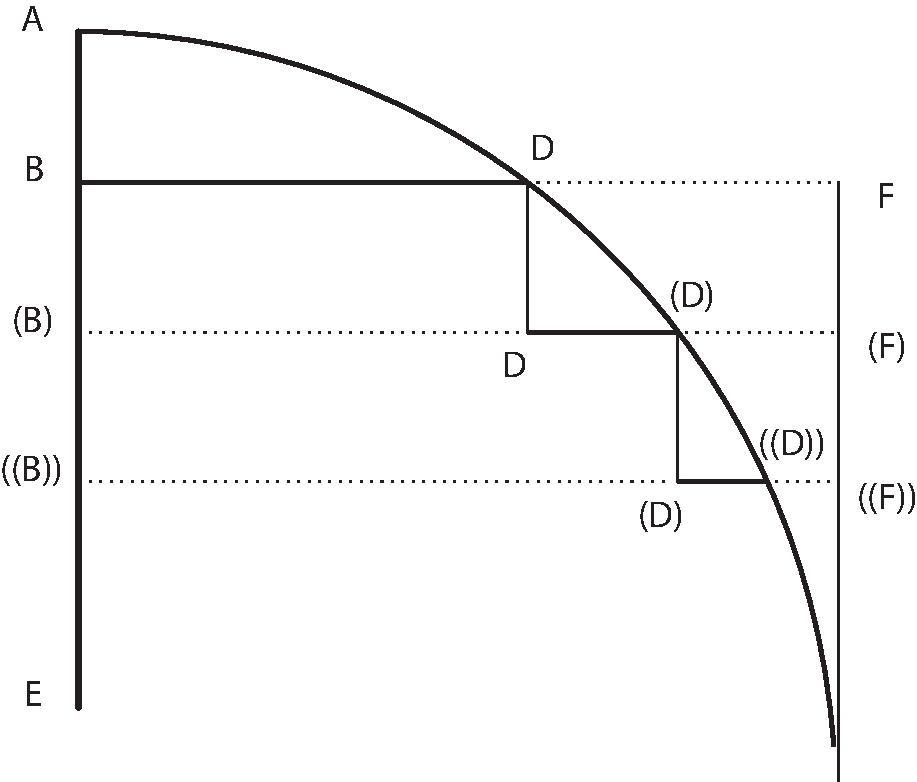
\includegraphics[width=0.64\textwidth]{images/lh0350911_013r_1-d1.pdf}\\
    \centering [\textit{Fig. 1}] %   \caption{Bildbeschreibung}
    %\end{wrapfigure}
    \pend
    \vspace{1.5em}
    \count\Bfootins=1000
\count\Cfootins=1200
\count\Afootins=1200
        \pstart
    \noindent
Soit \setline{1}dans la\textso{ 2. fig. }le point mobile port\'{e} en m\^{e}me temps par deux mouuemens,
dont l'un est uniforme, et dont la ligne de direction est $\displaystyle AE$, ou parallele
\edtext{\`{a} $\displaystyle AE$ comme $\displaystyle DD.$ $\displaystyle (D)(D)$. L'autre retard\'{e} egalement par les lieux o\`{u} il passe, dont la ligne de direction est $\displaystyle BF$ ou la parallele $\displaystyle (B)(F)$, $\displaystyle ((B))((F))$ etc.}{\lemma{\`{a} $\displaystyle AE$}\Bfootnote{\textit{(1)}\ l'autre retard\'{e} egalement par les lieux o\`{u} il passe, dont la ligne de direction est $\displaystyle BC$ \textit{(2)}\ comme  \textit{(a)}\ $\displaystyle D(C).$ $\displaystyle (D)((C))$ \textit{(b)}\ $\displaystyle DD.$ [...] $\displaystyle BF$ ou  \textbar\ la \textit{erg.}\ \textbar\ parallele [...] etc. \textit{L}}}
Ce qui se peut conceuuoir aisement en supposant qu'une regle
\edtext{inflexible}{\lemma{}\Bfootnote{inflexible \textit{erg.} \textit{L}}}
\edtext{$\displaystyle BF$ demeurant}{\lemma{}\Bfootnote{$\displaystyle BF$  \textbar\ regle \textit{gestr.}\ \textbar\ demeurant \textit{L}}}
tousjours parallele \`{a} elle m\^{e}me marche
[uniformement]\edtext{}{\Bfootnote{uniforment\textit{\ L \"{a}ndert Hrsg.}}}
le long de la droite
\edtext{immobile}{\lemma{}\Bfootnote{immobile \textit{erg.} \textit{L}}}
$\displaystyle AE$ et que
\edtext{cependant un autre mobile}{\lemma{cependant}\Bfootnote{\textit{(1)}\ le mobile \textit{(2)}\ un autre mobile \textit{L}}}
roule ou glisse sur cette regle
\edtext{$\displaystyle BF$}{\lemma{}\Bfootnote{$\displaystyle BF$ \textit{erg.} \textit{L}}},
d'un mouuement uniforme
\edtext{en soy}{\lemma{en}\Bfootnote{\textit{(1)}\ luy \textit{(2)}\ soy \textit{L}}}
m\^{e}me, mais
\edtext{retard\'{e} egalement en chaque endroit de la regle par le frottement}{\lemma{retard\'{e}}\Bfootnote{\textit{(1)}\ par le frottement de la regle, egalement en \textit{(2)}\ egalement [...] frottement. \textit{L}}}.
De sorte que le mobile va sur la regle de $\displaystyle B$ en $\displaystyle D$, ou de $\displaystyle D$ en $\displaystyle (D)$ ou de $\displaystyle (D)$ en $\displaystyle ((D))$
\edtext{jusqu'\`{a} ce qu'il s'arreste en $\displaystyle F$}{\lemma{jusqu'\`{a} [...] en $\displaystyle F$}\Bfootnote{\textit{erg.} \textit{L}}}[,]
pendant que la regle
\edtext{va de $\displaystyle A$ en $\displaystyle B$, ou de $\displaystyle B$ en $\displaystyle (B)$ ou}{\lemma{va}\Bfootnote{\textit{(1)}\ de $\displaystyle B$ en $\displaystyle (B)$ ou \textit{(2)}\ de $\displaystyle A$ [...] $\displaystyle (B)$ ou \textit{L}}}
de $\displaystyle (B)$ en
\edtext{$\displaystyle ((B))$. Or les parties de la ligne $\displaystyle AE$ s\c{c}avoir $\displaystyle AB$, $\displaystyle B(B)$, $\displaystyle (B)((B))$}{\lemma{$\displaystyle ((B))$.}\Bfootnote{\textit{(1)}\ Supposons \`{a} present que les dro \textit{(2)}\ Or les  \textit{(a)}\ portions  \textit{(b)}\ parties de  \textit{(aa)}\ l'espace $\displaystyle AE$  \textit{(bb)}\ la ligne [...] $\displaystyle (B)((B))$ \textit{L}}}
estant egales, et par consequent les espaces
\edtext{parcourus
[13~v\textsuperscript{o}] % \pend
par le mouuement uniforme, s\c{c}avoir $\displaystyle AB.$ $\displaystyle A(B)$. $\displaystyle A((B))$ estant en progression Arithmetique, les temps employez le seront aussi, par ce que dans le mouuement uniforme les temps employez sont uniformes aux espaces parcourus. Or}{\lemma{parcourus}\Bfootnote{\textit{(1)}\ par [13~v\textsuperscript{o}] 
 le mouuement uniforme,  \textbar\ $\displaystyle AB.$ $\displaystyle A(B).$ $\displaystyle A((B))$ \textit{erg.}\ \textbar\  estant en progression Arithmetique, les \textit{(2)}\ par avancement du mobile sur la regle, s\c{c}avoir $\displaystyle BD$, $\displaystyle D(D)$, $\displaystyle (D)((D))$ seront en progression Geometrique, car \textit{(3)}\ le \textit{(4)}\ d \textit{(5)}\ Or \textit{(6)}\ \textbar\ les espaces parcourus \textit{gestr.}\ \textbar\ par le [...] s\c{c}avoir $\displaystyle AB.$  \textit{(a)}\ etc.  \textit{(b)}\ $\displaystyle A(B).$ $\displaystyle A((B))$
 \textit{(aa)}\ sont en raison des temps employes; (:~par la definition du mouuement uniforme~:) et  \textit{(bb)}\ estant en [...] parcourus. Or \textit{L}}}
les temps employez estant en progression Arithmetique,
les espaces qui restent \`{a} parcourir dans la regle, jusqu'au point de repos,
s\c{c}avoir $\displaystyle DF$, $\displaystyle (D)(F)$, $\displaystyle ((D))((F))$
seront en progression Geometrique par
le\edtext{\textso{ theor. 5. }Donc les espaces \`{a} parcourir par le mouuement uniforme de la regle, estant en progression arithmetique, les espaces \`{a} parcourir par le mouuement retard\'{e} sur la regle m\^{e}me seront en progression geometrique. Le m\^{e}me se}{\lemma{\textso{theor. 5.}}\Bfootnote{\textit{(1)}\ Et le m\^{e}me se \textit{(2)}\ Donc les [...] uniforme  \textbar\ de la regle \textit{erg.}\ \textbar\ , estant [...] retard\'{e}  \textit{(a)}\ dans  \textit{(b)}\ sur la [...] Le m\^{e}me se \textit{L}}}
trouuant \edtext{veritable, les intervalles $\displaystyle B(B).$ $\displaystyle (B)((B))$,
ou $\displaystyle F(F).$ $\displaystyle (F)((F))$
estant moindres qu'aucune ligne donn\'{e}e; le lieu}%
{\lemma{veritable,}\Bfootnote{%
\textit{(1)}\ quelques petits que %
\textit{(2)}\ les intervalles $\displaystyle B(B).$ %
\textit{(a)}\ ou %
\textit{(b)}\ $\displaystyle (B)((B))$, ou [...] donn\'{e}e; %
\textit{(aa)}\ la ligne %
\textit{(bb)}\ le lieu \textit{L}}}
$\displaystyle A D (D) ((D))$
qui passe par toutes les terminations des lignes Geometriquement proportionnelles,
et egalement distantes entre elles,
$\displaystyle FD.$ $\displaystyle (F)(D).$ $\displaystyle ((F))((D))$
\edtext{sera la ligne Logarithmique par la definition de cette courbe.\protect\\
\hspace*{7,5mm}Q.E.D.}{\lemma{sera}\Bfootnote{\textit{(1)}\ Logarithmique. Ce qu'il falloit demonstrer. \textit{(2)}\ la  \textit{(a)}\ courbe  \textit{(b)}\ ligne Logarithmique  \textbar\ ( \textit{gestr.}\ \textbar\ par la [...] Q.E.D. \textit{L}}}
\pend
\count\Bfootins=1500
\count\Cfootins=1500
\count\Afootins=1500
\newpage